\documentclass[12pt, a4paper]{article}

% --- Formatting according to 3YP Handbook 2025/26 ---
\usepackage{iftex}
\usepackage[margin=2cm]{geometry}
\usepackage{setspace}
\onehalfspacing

\ifPDFTeX
    \usepackage[T1]{fontenc}
    \usepackage[utf8]{inputenc}
    \usepackage{helvet}
    \renewcommand{\familydefault}{\sfdefault}
\else
    \usepackage{fontspec}
    \defaultfontfeatures{Ligatures=TeX}
    \setmainfont{Carlito}
    \setsansfont{Carlito}
\fi

\usepackage{graphicx}
\usepackage{adjustbox}
\usepackage{amsmath, amssymb, amsfonts}
\usepackage{tikz}
\usetikzlibrary{arrows.meta, positioning, shapes.geometric, calc, fit, backgrounds, decorations.pathreplacing, shadows.blur}
\usepackage{caption}
\usepackage{booktabs}
\usepackage{multirow}
\usepackage{hyperref}
\usepackage{array}
\usepackage{xcolor}
\usepackage{soul}

\sethlcolor{yellow}
\definecolor{meetingBlue}{RGB}{226, 239, 255}
\definecolor{meetingBlueBorder}{RGB}{70, 105, 170}
\newcommand{\mnote}[1]{%
    \par\smallskip
    \noindent\fcolorbox{meetingBlueBorder}{meetingBlue}{%
        \parbox{0.96\linewidth}{\footnotesize\textbf{Meeting note:} #1}%
    }%
    \par\smallskip
}

\begin{document}

\raggedright

\begin{titlepage}
    \centering
    \vspace*{3cm}
    {\LARGE \textbf{A Brain-Computer Interface Control \\ System Design Based on Deep Learning}\par}
    \vspace{1.5cm}
    {\Large Third Year Individual Project -- Final Report\\v12 Meeting Annotated Version\par}
    \vspace{2.5cm}
    {\large April 2026\par}
    \vspace{2cm}
    {\large Student ID: 11314389\par}
    \vfill
    {\large Academic Advisor: Alex Casson\par}
\end{titlepage}

\pagenumbering{roman}
\setcounter{page}{2}

\begin{singlespace}
\tableofcontents
\end{singlespace}
\clearpage

\phantomsection
\section*{Abstract}
\addcontentsline{toc}{section}{Abstract}
Motor imagery (MI) Brain-Computer Interfaces (BCIs) remain difficult to deploy for real-world robotic control because existing approaches treat EEG decoding as a static, open-loop classification problem and depend on high-density electrode arrays. This project presents a closed-loop BCI control pipeline that addresses these limitations through three contributions: (1)~a hybrid CNN and Transformer classifier (EEGTransformer) that captures both the spatial specificity and long-range temporal structure of MI signals; (2)~a Deep Q-Network (DQN) reinforcement learning agent that compensates for transient classification errors by \hl{aggregating classifier evidence over time}; and (3)~a systematic channel reduction study that maps the 64-channel laboratory setup down to an 8-channel configuration compatible with consumer-grade OpenBCI hardware. Furthermore, an evaluation of Independent Component Analysis (ICA) \hl{showed limited benefit} for motor imagery preprocessing, leading to the adoption of a bandpass-only pipeline.
\mnote{Changed stronger wording to a more evidence-aligned description. ``Aggregating classifier evidence'' is more precise than implying a biological or temporal integration claim that was not directly measured, and ``showed'' avoids overstating the ICA result.}

Evaluated across BCI Competition IV-2a (22-channel, 4-class), IV-2b (3-channel, 2-class), and PhysioNet EEGMMIDB (64-channel, 109 subjects), the EEGTransformer achieved mean accuracies of 73.80\%, 82.87\%, and 88.78\% (with subject-specific fine-tuning), respectively. The channel reduction study identified C3 as the most critical electrode and showed that an 8-channel subset retains 72.54\% accuracy after fine-tuning. An end-to-end simulation demonstrated that the DQN agent achieves a 99\% target reach rate even when driven by imperfect EEG classifications (82\% accuracy), confirming that closed-loop RL effectively compensates for decoder errors. \hl{EEG classification was evaluated offline using pre-recorded datasets, while control evaluation was conducted in simulation}, as this undergraduate project does not have University of Manchester ethical approval for live human subject testing.
\mnote{Added the offline/simulation boundary in the Abstract so a reader immediately understands the validation scope and does not infer live human-subject OpenBCI testing.}
\clearpage

\phantomsection
\section*{Declaration of Originality}
\addcontentsline{toc}{section}{Declaration of Originality}
I hereby confirm that this dissertation is my own original work unless referenced clearly to the contrary, and that no portion of the work referred to in the dissertation has been submitted in support of an application for another degree or qualification of this or any other university or other institute of learning.
\clearpage

\phantomsection
\section*{Intellectual Property Statement}
\addcontentsline{toc}{section}{Intellectual Property Statement}
\begin{enumerate}
    \item The author of this report, including any appendices, owns certain copyright or related rights in it and has granted The University of Manchester rights to use such copyright for administrative purposes.
    \item Copies of this report, whether in full or in extracts and whether in hard or electronic form, may be made only in accordance with the Copyright, Designs and Patents Act 1988, as amended, and any licensing agreements or regulations issued by the University from time to time. This page must form part of any such copies made.
    \item The ownership of certain copyright, patents, designs, trademarks, and other intellectual property described in this report, together with any reproductions of copyright works such as figures or tables, may not belong to the author and may instead belong to third parties. Such material must not be made available for use without the prior written permission of the relevant owner.
    \item Further information on the conditions under which disclosure, publication, and commercialisation of this report, its copyright, and any related intellectual property may take place is available in the University of Manchester intellectual-property policy and the University Library regulations.
\end{enumerate}
\clearpage

\phantomsection
\section*{Acknowledgements}
\addcontentsline{toc}{section}{Acknowledgements}
The author thanks Alex Casson for feedback on the report draft and for weekly technical discussions throughout the project. Public benchmark datasets, open-source scientific software, and the University computing environment were essential to the completion of this work.
\clearpage

\pagenumbering{arabic}
\setcounter{page}{1}

%=============================================================================
\section{Introduction}
%=============================================================================

%-----------------------------------------------------------------------------
\subsection{Background and Motivation}
%-----------------------------------------------------------------------------

Electroencephalography (EEG) is a non-invasive neuroimaging technique that records the electrical activity of the brain through electrodes placed on the scalp. When large populations of cortical neurons fire synchronously, they generate voltage fluctuations on the order of microvolts ($\mu$V), which surface electrodes can detect with millisecond temporal resolution. EEG is widely used in clinical neuroscience for diagnosing epilepsy, sleep disorders, and other neurological conditions, and has become the predominant recording modality for Brain-Computer Interfaces (BCIs) because of its portability, low cost, and high temporal resolution relative to other neuroimaging techniques such as functional magnetic resonance imaging (fMRI) or magnetoencephalography (MEG)~\cite{hameed2025enhancing}.

A Brain-Computer Interface (BCI) is a system that translates neural signals directly into commands for external devices, bypassing the body's normal neuromuscular output pathways. BCIs offer a communication and control channel for individuals with severe motor disabilities---such as amyotrophic lateral sclerosis (ALS), spinal cord injury, or locked-in syndrome---who cannot use conventional interfaces. Beyond assistive technology, BCIs are increasingly explored for rehabilitation, gaming, and hands-free device control~\cite{jeong2020multimodal}.

Motor Imagery (MI) is a mental process in which an individual imagines performing a movement (e.g., clenching the left hand, moving the right foot) without actually executing it. During MI, the sensorimotor cortex produces characteristic changes in neural oscillations known as Event-Related Desynchronisation (ERD) and Event-Related Synchronisation (ERS). Specifically, imagining a movement of one limb causes a suppression (ERD) of the Mu rhythm (8--13\,Hz) and Beta rhythm (13--30\,Hz) over the contralateral motor cortex, and a simultaneous enhancement (ERS) over the ipsilateral cortex. These spatially and spectrally specific patterns provide the neural signatures that MI-BCI systems exploit for classification~\cite{hameed2025enhancing}.

MI-based BCIs are particularly attractive because they require no external stimulation (unlike P300 or SSVEP paradigms) and rely entirely on the user's voluntary mental activity. However, translating MI-BCI systems into reliable, real-time robotic controllers remains an open problem driven by three fundamental challenges:

\textbf{Signal non-stationarity.}\quad EEG patterns shift across sessions, days, and subjects due to variations in electrode impedance, fatigue, and cognitive strategy~\cite{hameed2025enhancing}. A decoder calibrated on one recording session therefore degrades when applied to subsequent sessions or new users, limiting the practical lifespan of static models.

\textbf{Open-loop control constraints.}\quad Conventional BCI pipelines operate in open loop. Each classified epoch is mapped to a fixed command, meaning the system cannot recover from a misclassification once it occurs. In robotic manipulation, where smooth, corrective trajectories are essential, a single erroneous command can destabilise an entire motion sequence.

\textbf{Hardware scalability.}\quad Most high-performing MI decoders are developed on 64-channel research-grade amplifiers, yet portable deployment requires consumer-grade devices such as the OpenBCI Cyton (8 channels). Naively discarding channels forfeits the spatial information on which these decoders depend. Therefore, channel reduction requires an empirical estimate of which electrodes carry the most discriminative signal.

%-----------------------------------------------------------------------------
\subsection{Aims and Objectives}
%-----------------------------------------------------------------------------

The overall aim of this project is to \textbf{design, implement, and validate a closed-loop Brain-Computer Interface control system} that translates motor imagery EEG signals into robotic arm commands using deep learning and reinforcement learning, while remaining deployable on consumer-grade hardware.

To achieve this aim, five objectives are pursued. On the classification side, the project develops a hybrid CNN-Transformer architecture (EEGTransformer) that combines convolutional spatial filtering with Transformer-based temporal modelling, evaluated across BCI Competition IV-2a, IV-2b, and PhysioNet EEGMMIDB to assess generalisation across electrode densities, class counts, and subject populations. A two-stage transfer learning strategy, comprising cross-subject pre-training followed by subject-specific fine-tuning, is implemented to bridge the cross-subject generalisation gap while minimising per-user calibration burden. A systematic channel reduction study uses ablation-based importance analysis to identify an 8-channel electrode subset compatible with the OpenBCI Cyton and quantify the trade-off between channel count and classification accuracy.

On the control side, a closed-loop Deep Q-Network (DQN) reinforcement learning agent integrates noisy MI predictions over time and learns corrective motor policies, decoupling control success from instantaneous classification accuracy. Finally, the complete end-to-end pipeline, spanning EEG acquisition, preprocessing, classification, RL control, and robotic actuation, is evaluated in simulation under imperfect EEG decoding conditions.

%-----------------------------------------------------------------------------
\subsection{Proposed Approach}
%-----------------------------------------------------------------------------

These limitations motivate a system that combines complementary strengths, and this project contributes in three areas.

At the classification level, an EEGTransformer architecture pairs an EEGNet-inspired convolutional front-end with a multi-layer Transformer encoder. The convolutional stage provides the spatial inductive biases that pure Transformers lack, while the Transformer captures the long-range temporal dependencies that CNNs and Common Spatial Patterns (CSP) miss. This combination retains the data-driven spatial filtering of EEGNet while adding global temporal context, addressing the single-trial isolation problem of purely convolutional models without incurring the training instability of recurrent neural networks (RNNs).

At the control level, rather than treating classification as the final output, a DQN agent consumes the classifier's predictions as part of a richer state representation and learns to produce corrective motor commands through reward-driven policy optimisation. By aggregating evidence over multiple time steps, the agent can override transient misclassifications, directly addressing the open-loop fragility of conventional pipelines.

At the deployment level, a systematic ablation study quantifies each electrode's contribution to classification, enabling evidence-based selection of an 8-channel subset compatible with the OpenBCI Cyton. Combined with subject-specific fine-tuning from a pre-trained 64-channel model, this strategy preserves practical classification performance while reducing hardware cost and setup complexity by an order of magnitude.

The system is validated across three datasets that collectively span different electrode montages (3, 22, 64 channels), class counts (2, 4), and subject pools (9--109). End-to-end control is evaluated in simulation using pre-recorded EEG data and PyBullet robotic arm simulation.

%-----------------------------------------------------------------------------
\subsection{Report Structure}
%-----------------------------------------------------------------------------

The remainder of the report is organised as follows. Chapter~2 reviews the main MI-EEG classification paradigms, representative benchmark datasets, and the gap addressed by this project. Chapter~3 describes the methods, including dataset handling, preprocessing, EEGTransformer design, training protocol, channel-reduction procedure, and the RL control formulation. Chapter~4 presents the experimental results and discusses their implications for classification accuracy, channel efficiency, preprocessing design, and closed-loop control. Chapter~5 summarises how the project was planned and managed. Chapter~6 concludes the report and outlines the most relevant directions for future work.

%=============================================================================
\section{Literature Review}
%=============================================================================

%-----------------------------------------------------------------------------
\subsection{Introduction}
%-----------------------------------------------------------------------------

This chapter surveys existing approaches to MI-EEG classification and the datasets commonly used for evaluation, situating the current project within the broader research landscape.

%-----------------------------------------------------------------------------
\subsection{MI Classification Methods}
%-----------------------------------------------------------------------------

\textbf{Classical spatial filtering.}\quad The dominant classical pipeline extracts Common Spatial Patterns (CSP) features and classifies them with Linear Discriminant Analysis (LDA)~\cite{hameed2025enhancing}. CSP maximises the variance ratio between classes, producing compact spatial filters that are neurophysiologically interpretable. However, CSP assumes that the covariance structure of the data is stationary across trials, an assumption violated by session-to-session drift. As a result, CSP+LDA performance degrades rapidly without frequent recalibration. Filter Bank CSP (FBCSP)~\cite{ang2008fbcsp} extends CSP by applying multiple frequency sub-bands and selecting the most discriminative features, achieving improved robustness at the cost of higher computational complexity.

\textbf{Convolutional neural networks.}\quad To relax the stationarity assumption, convolutional architectures such as EEGNet~\cite{lawhern2018eegnet} and ShallowConvNet~\cite{schirrmeister2017deep} learn spatial--temporal filters directly from data. EEGNet introduced depthwise and separable convolutions for compact EEG feature extraction, achieving 68--72\% on standard 4-class benchmarks. ShallowConvNet applies temporal and spatial convolutions with log-variance pooling to capture band-power features. Yet these models process each trial independently: they lack any mechanism to carry information across successive epochs, making them susceptible to isolated noisy trials.

\textbf{Recurrent architectures.}\quad Recurrent networks (LSTMs, GRUs) address this limitation by maintaining hidden states across time steps, enabling sequential modelling of EEG dynamics. In practice, however, their performance on long MI epochs is hampered by vanishing gradients and sensitivity to sequence length, and their strictly sequential computation prevents parallelisation during training~\cite{vaswani2017attention}.

\textbf{Transformer-based models.}\quad Transformers overcome the sequential bottleneck of RNNs through self-attention, modelling arbitrary pairwise dependencies in a single forward pass. EEG-Conformer~\cite{song2022eeg} combines convolutional modules with Transformer encoders for MI classification, achieving state-of-the-art results. ATCNet~\cite{altaheri2022atcnet} combines attention-based temporal convolutional networks with sliding window augmentation. EEG-TCNet~\cite{ingolfsson2020eeg} proposes a compact temporal convolutional architecture as an efficient alternative. Their weakness relative to CNNs is the opposite: pure self-attention lacks the spatial inductive biases that make EEGNet effective.

\textbf{Reinforcement learning in BCI.}\quad A separate line of work applies RL to BCI, but primarily for offline feature selection. MARS~\cite{shin2024mars} uses multi-agent RL to optimise spatial, spectral, and temporal filter banks. RLEEGNet~\cite{nallani2024rleegnet} formulates EEG decoding within an MDP framework. However, neither system closes the loop with a physical actuator.

Table~\ref{tab:lit_methods} summarises representative MI classification methods and their reported performance on the BCI Competition IV-2a benchmark.

\begin{table}[htbp]
\centering
\caption{Comparison of MI-EEG classification methods on BCI Competition IV-2a (4-class, 22-channel). Results are mean subject-dependent accuracies (\%) unless otherwise noted.}
\label{tab:lit_methods}
\begin{tabular}{@{} l l c l @{}}
\toprule
\textbf{Method} & \textbf{Architecture Type} & \textbf{Accuracy (\%)} & \textbf{Reference} \\
\midrule
CSP + LDA           & Spatial filtering + linear      & 60--68   & \cite{hameed2025enhancing} \\
FBCSP + SVM         & Filter bank + classifier        & 67.6     & \cite{ang2008fbcsp} \\
ShallowConvNet      & Temporal--spatial CNN            & 68--71   & \cite{schirrmeister2017deep} \\
EEGNet              & Depthwise separable CNN          & 68--72   & \cite{lawhern2018eegnet} \\
FBCNet              & Filter-bank + CNN               & 76.2     & \cite{mane2021fbcnet} \\
EEG-TCNet           & Temporal convolutional           & 77.4     & \cite{ingolfsson2020eeg} \\
EEG-Conformer       & CNN + Transformer                & 77.7     & \cite{song2022eeg} \\
ATCNet              & Attention temporal conv.         & 80.5     & \cite{altaheri2022atcnet} \\
\midrule
\textbf{EEGTransformer (Ours)} & \textbf{CNN + Transformer} & \textbf{73.80} & \textbf{This work} \\
\bottomrule
\end{tabular}
\end{table}

As shown in Table~\ref{tab:lit_methods}, purely convolutional approaches (EEGNet, ShallowConvNet) typically achieve 68--72\%, while hybrid CNN-Transformer architectures (EEG-Conformer, ATCNet) push accuracy above 77\%. The EEGTransformer proposed in this project achieves 73.80\%, which is competitive with established CNN baselines and supports the use of a hybrid CNN-Transformer design. Direct comparison across studies is complicated by differences in preprocessing, data augmentation, and evaluation protocols.

%-----------------------------------------------------------------------------
\subsection{Datasets Used in MI-BCI Research}
%-----------------------------------------------------------------------------

The choice of evaluation dataset significantly influences the reported results and the generalisability of conclusions. Table~\ref{tab:lit_datasets} provides a comparative overview of the three datasets used in this study, together with their prevalence in the MI-BCI literature and their respective advantages and limitations.

\begin{table}[htbp]
\centering
\caption{Comparison of MI-EEG benchmark datasets: characteristics, usage prevalence, and limitations.}
\label{tab:lit_datasets}
\begin{tabular}{@{} >{\raggedright\arraybackslash}p{2.8cm} c c c >{\raggedright\arraybackslash}p{3.5cm} >{\raggedright\arraybackslash}p{3.5cm} @{}}
\toprule
\textbf{Dataset} & \textbf{Ch.} & \textbf{Classes} & \textbf{Subjects} & \textbf{Advantages} & \textbf{Limitations} \\
\midrule
BCI Competition IV-2a~\cite{tangermann2012bci} & 22 & 4 & 9 & Most widely cited MI benchmark; standardised evaluation protocol; 4-class task enables multi-class comparison & Small subject pool (9); limited demographic diversity; may overfit to benchmark \\[6pt]
BCI Competition IV-2b~\cite{tangermann2012bci} & 3 & 2 & 9 & Tests minimal-channel performance; binary task is clinically relevant & Only 3 channels; 2-class task is less challenging; same 9 subjects as 2a \\[6pt]
PhysioNet EEGMMIDB~\cite{goldberger2000physiobank} & 64 & 4 & 109 & Large subject pool enables cross-subject studies; high channel density; freely accessible & Inconsistent recording quality across subjects; some subjects show minimal MI responses; no standardised training/test split \\
\bottomrule
\end{tabular}
\end{table}

BCI Competition IV-2a is by far the most widely used benchmark in the MI-BCI literature, with hundreds of published results enabling direct methodological comparison. Its 4-class paradigm (left hand, right hand, feet, tongue) provides a rigorous multi-class test, but its small participant pool (9 individuals) limits the statistical power of cross-subject analyses.

BCI Competition IV-2b uses only 3 bipolar EEG channels and a binary left/right hand task, making it valuable for evaluating algorithms under extreme channel scarcity---a scenario directly relevant to consumer-grade BCI deployment.

PhysioNet EEGMMIDB offers the largest publicly available MI dataset (109 participants, 64 channels), enabling large-scale cross-participant generalisation studies that are infeasible with 9-participant datasets. However, recording quality varies across participants, and the absence of a standardised training/test partition complicates cross-study comparison. Despite these limitations, PhysioNet's scale makes it particularly useful for training data-hungry deep learning models and for evaluating transfer learning strategies.

By evaluating across all three datasets, this project tests generalisability along three independent axes: electrode density (3 vs.\ 22 vs.\ 64 channels), classification difficulty (2 vs.\ 4 classes), and population diversity (9 vs.\ 109 subjects).

\textbf{\hl{Why these datasets were selected instead of other public EEG datasets.}}\quad Many public EEG resources are available, but not all are equally suitable for this project's research questions. The chosen datasets had to satisfy four practical requirements simultaneously: they had to be openly accessible, genuinely focused on motor imagery rather than other EEG paradigms, sufficiently established in the literature to support comparison, and \hl{complementary in montage size and evaluation role}. BCI~IV-2a was retained because it remains the standard 4-class benchmark used for direct comparison with prior MI classifiers. BCI~IV-2b was retained because its 3-channel setup provides a realistic minimal-channel stress test relevant to consumer BCI deployment. PhysioNet EEGMMIDB was retained because it is the only dataset in this project large enough to support meaningful cross-subject pre-training and transfer-learning analysis at scale. Other candidate datasets could have been added, but many would mainly duplicate one of these roles or introduce additional paradigm differences without strengthening the central comparison. For that reason, this project prioritised a deliberately complementary three-dataset set rather than a larger but less focused collection.
\mnote{New justification added after supervision feedback: it explains why the report uses three targeted public datasets instead of appearing to ignore other available EEG datasets.}

%-----------------------------------------------------------------------------
\subsection{From Literature to System Structure}
%-----------------------------------------------------------------------------

The literature reviewed above motivates more than a standalone classifier. In most prior work, EEG preprocessing, MI decoding, and robotic control are studied as separate modules; classification papers often stop at predicted labels, while control papers frequently assume a reliable intention signal already exists. \hl{This project instead combines these strands into a closed-loop structure.} Conceptually, the system has three stages: signal preparation, intention decoding, and action selection. Raw EEG must first be filtered and segmented into epochs that retain task-relevant Mu/Beta activity; a decoder must then convert those epochs into class evidence; and a controller must finally interpret that evidence in the context of the robot's current state so that occasional misclassifications do not immediately cause task failure.

\hl{This interpretation is important for reading the architecture diagram that appears at the start of Chapter~3.} That figure is not introducing an unrelated block diagram; rather, it summarises how the different research strands identified in this chapter are connected in the present project. Its left-hand group corresponds to the preprocessing literature, its middle group corresponds to the hybrid CNN--Transformer decoding literature, and its right-hand group corresponds to sequential control and RL-based decision making. Presenting the system in this modular way makes clear why the project cannot be evaluated solely as an open-loop classification benchmark: the intended contribution is the integration of these stages into a single BCI-to-control pipeline.
\mnote{New bridge section added so the Literature Review now prepares the reader for the architecture diagram and frames the project as an integrated BCI-to-control pipeline, not just a classifier benchmark.}

%-----------------------------------------------------------------------------
\subsection{Summary}
%-----------------------------------------------------------------------------

The literature indicates that strong MI decoders must balance spatial inductive bias, temporal modelling capacity, and robustness to subject variability. It also shows that no single benchmark captures all deployment-relevant conditions. These observations motivate the hybrid EEGTransformer design and the multi-dataset evaluation protocol adopted in the next chapter.

%=============================================================================
\section{Methods}
%=============================================================================

%-----------------------------------------------------------------------------
\subsection{Introduction}
%-----------------------------------------------------------------------------

This chapter defines the experimental procedures used in the project. The emphasis is on reproducibility: datasets, preprocessing choices, model configurations, optimisation settings, evaluation splits, and the control formulation are specified here, while numerical outcomes are deferred to Chapter~4.

The system is organised into three visual groups that \hl{correspond to four functions}: EEG preprocessing, deep learning classification, reinforcement learning control, and hardware integration. In Figure~\ref{fig:system_overview}, hardware integration is shown through the BrainFlow/OpenBCI acquisition interface and the serial SO-101 control interface.

\hl{Before reading the figure, it is useful to state explicitly what each group represents.} The first group takes raw EEG and converts it into filtered, fixed-length epochs suitable for learning. The second group is the EEGTransformer itself, which maps each epoch to class evidence by combining convolutional spatial filtering with Transformer-based temporal modelling. The third group is the closed-loop controller, which receives both robot-state information and classifier output, then chooses a control action rather than directly executing the raw class prediction. The diagram should therefore be read from left to right as an information-processing chain: \emph{signal} $\rightarrow$ \emph{decoded intention} $\rightarrow$ \emph{control decision}. This ordering is central to the project because it explains why classifier accuracy alone is not the only relevant performance measure.
\mnote{Methods opening was clarified to make Figure 3 self-explanatory. The wording avoids a vague ``three groups realise four functions'' claim and spells out how to read the pipeline.}

\begin{figure}[htbp]
    \centering
    \begin{adjustbox}{max width=1.15\textwidth,center}
                % --- DeepMind / OpenAI-style clean pastel palette ---
    \definecolor{bgGray}{RGB}{246, 247, 249}
    \definecolor{borderGray}{RGB}{184, 188, 194}
    \definecolor{textMain}{RGB}{42, 46, 52}
    \definecolor{textMuted}{RGB}{93, 100, 110}

    \definecolor{blueFill}{RGB}{233, 240, 247}
    \definecolor{blueBorder}{RGB}{160, 181, 201}

    \definecolor{greenFill}{RGB}{233, 242, 236}
    \definecolor{greenBorder}{RGB}{160, 184, 169}

    \definecolor{orangeFill}{RGB}{247, 239, 231}
    \definecolor{orangeBorder}{RGB}{205, 178, 154}

    \definecolor{purpleFill}{RGB}{239, 235, 244}
    \definecolor{purpleBorder}{RGB}{176, 164, 196}


\begin{tikzpicture}[
    >=latex,
    % Box styles (Flat, No Shadows)
    nodeBox/.style={
        rectangle, rounded corners=6pt, draw=#1Border, fill=#1Fill, thick,
        align=center, text=textMain, inner sep=7pt, minimum width=3.0cm, minimum height=1.3cm
    },
    noteBox/.style={
        rectangle, rounded corners=6pt, draw=borderGray, thick, fill=white,
        align=left, text=textMain, inner sep=6pt, text width=3.4cm
    },
    groupBox/.style={
        rectangle, rounded corners=12pt, draw=borderGray, thick, dashed, inner sep=10pt, fill=bgGray
    },
    % Arrow styles
    arr/.style={->, >={Stealth[length=2.5mm, width=1.5mm]}, thick, textMain},
    arrDashed/.style={->, >={Stealth[length=2.5mm, width=1.5mm]}, thick, dashed, textMuted},
    % Text styles
    lbl/.style={font=\normalsize, text=textMuted, align=center, fill=none, inner sep=3pt, midway, above=2pt, sloped},
    lblWhite/.style={font=\normalsize, text=textMuted, align=center, fill=none, inner sep=3pt, midway, above=2pt, sloped},
    lblFlat/.style={font=\normalsize, text=textMuted, align=center, fill=none, inner sep=3pt, midway, above=2pt},
    lblWhiteFlat/.style={font=\normalsize, text=textMuted, align=center, fill=none, inner sep=3pt, midway, above=2pt},
    lblCenter/.style={font=\normalsize, text=textMuted, align=center, fill=none, inner sep=1pt},
    noteText/.style={font=\footnotesize, text=textMuted, align=left},
    title/.style={font=\normalsize\bfseries, text=textMain, anchor=south}
]

% ==========================================
% PILLAR 1: Signal Pipeline
% ==========================================
\node[nodeBox=blue] (eeg) at (0, 0) {
    \textbf{EEG Acquisition}\\
    \footnotesize OpenBCI (8-ch) $\vert$ PhysioNet (64-ch)
};
\node[title, above=0.4cm of eeg] (p1_title) {1. EEG Processing};

\node[nodeBox=green, below=0.8cm of eeg] (preproc) {
    \textbf{Preprocessing}\\
    \footnotesize Bandpass (8--30\,Hz) $\to$ Fixed-Length Epochs
};
\draw[arr] 
(eeg) -- (preproc);
\node[lblCenter] at ($(eeg.south)!0.5!(preproc.north)$) {Raw Signal};

\node[rectangle, rounded corners=6pt, draw=borderGray, thick, fill=white, align=center, text=textMain, inner sep=8pt, minimum width=3.7cm, minimum height=1.4cm, below=0.8cm of preproc] (baseline) {
    \textbf{Baseline Classifier}\\
    \footnotesize OVR-CSP + LDA
};
\draw[arrDashed] 
(preproc) -- (baseline);
\node[lblCenter] at ($(preproc.south)!0.5!(baseline.north)$) {Comparison};

\begin{scope}[on background layer]
    \node[groupBox, fit=(p1_title) (eeg) (preproc) (baseline)] (group1) {};
\end{scope}

% ==========================================
% PILLAR 2: EEGTransformer
% ==========================================

% Convolutional Front-End
\node[nodeBox=orange] (cnn) at (7.5, 0 |- eeg.north) [anchor=north] {
    \textbf{Convolutional Front-End}\\
    \footnotesize Temporal $\to$ Spatial $\to$ Separable
};
\node[title, above=0.4cm of cnn] (p2_title) {2. EEGTransformer Model};

% Patch Embeddings
\node[nodeBox=orange, below=0.8cm of cnn] (patch) {
    \textbf{Patch Embeddings}\\
    \footnotesize Spatiotemporal Tokenization
};

% Transformer
\node[nodeBox=orange, below=0.8cm of patch] (trans) {
    \textbf{Transformer Encoder}\\
    \footnotesize Multi-Head Self-Attention
};

% Fusion & Head
\node[nodeBox=orange, below=0.8cm of trans] (fuse) {
    \textbf{Residual Fusion}\\
    \footnotesize CNN Features $\oplus$ Global Context
};

% Arrows for Pillar 2
% Filtered Epochs Arrow
\coordinate (P1) at ($ (preproc.east) + (0.8, 0) $);
\draw[arr] 
(preproc.east) -- (P1)
-- node[lblWhite, xshift=0.5cm] {Filtered Epochs}
(P1 |- cnn.west)
-- (cnn.west);

\draw[arr] (cnn) -- (patch);
\draw[arr] (patch) -- (trans);
\draw[arr] (trans) -- (fuse);

% Residual Arrow on the LEFT, rectangular
\coordinate (P4) at ($ (patch.west) + (-1.1, 0) $);
\draw[arr] (patch.west) -- (P4) -- node[lblWhite] {Residual} (P4 |- fuse.west) -- (fuse.west);

\begin{scope}[on background layer]
    \node[groupBox, fit=(p2_title) (cnn) (fuse)] (group2) {};
\end{scope}

% ==========================================
% PILLAR 3: RL Control
% ==========================================

% State
\node[nodeBox=purple] (state) at (15.0, 0 |- eeg.north) [anchor=north] {
    \textbf{State Representation} $s_t$\\
    \footnotesize Kinematics $\oplus$ Classifier Output
};
\node[title, above=0.4cm of state] (p3_title) {3. Closed-Loop RL Control};

% RL Agent
\node[nodeBox=purple, below=0.8cm of state] (agent) {
    \textbf{DQN Agent}\\
    \footnotesize Transformer / CNN+LSTM Q-Net
};

% Environment
\node[nodeBox=purple, below=0.8cm of agent] (env) {
    \textbf{Robotic Environment}\\
    \footnotesize SO-101 Arm Manipulation
};

% Arrows for Pillar 3
\coordinate (P2) at ($ (fuse.east) + (1.0, 0) $);
\draw[arr] (fuse.east) -- (P2) -- node[lblWhite] {Predicted Class\\\& Confidence} (P2 |- state.west) -- (state.west);

\draw[arr] (state) -- (agent);
\draw[arr] 
(agent) -- (env);
\node[lblCenter] at ($(agent.south)!0.5!(env.north)$) {Action $a_t$};


% Feedback loop
\coordinate (P3) at ($ (env.east) + (2.0, 0) $);
\draw[arr] (env.east) -- (P3) -- node[lblWhite] {Next State $s_{t+1}$\\\& Reward $r_t$} (P3 |- state.east) -- (state.east);

% Deployment notes
\node[noteBox, below=0.9cm of env] (hardware) {
    \textbf{Hardware Integration}\\
    \textcolor{textMuted}{BrainFlow $\rightarrow$ OpenBCI}\\
    \textcolor{textMuted}{Serial Protocol $\rightarrow$ SO-101 (Feetech STS3215)}
};
\node[noteText, below=0.3cm of hardware, anchor=north] (commands) {4-class MI $\rightarrow$ 4 commands: left, right, up, down};

\begin{scope}[on background layer]
    \node[groupBox, fit=(p3_title) (state) (env)] (group3) {};
\end{scope}

\end{tikzpicture}
    \end{adjustbox}
    \caption{\textbf{System Architecture Overview.} The pipeline is shown as three visual groups spanning four functions: EEG processing, deep learning classification, reinforcement learning control, and hardware integration. Raw EEG is preprocessed, then classified by the EEGTransformer. The predicted MI class and confidence form part of the state observed by a DQN agent, whose action $a_t$ drives the robotic environment. In the control setting used here, 4-class MI predictions are mapped to four directional commands (left, right, up, down), while hardware integration is handled through the BrainFlow/OpenBCI acquisition interface and the serial SO-101 control interface.}
    \label{fig:system_overview}
\end{figure}

%-----------------------------------------------------------------------------
\subsection{Datasets}
%-----------------------------------------------------------------------------

Three datasets were used, but they were not merged into a single training corpus. Instead, each was processed and evaluated independently because the montages, class definitions, and published protocols differ. Table~\ref{tab:datasets_v10} summarises the dataset properties and the protocol used for each part of the project.

\begin{table}[htbp]
\centering
\caption{Datasets used in this study and the associated evaluation protocol.}
\label{tab:datasets_v10}
\begin{tabular}{@{} >{\raggedright\arraybackslash}p{2.5cm} c c c c >{\raggedright\arraybackslash}p{4.3cm} @{}}
\toprule
\textbf{Dataset} & \textbf{EEG Ch.} & \textbf{$f_s$ (Hz)} & \textbf{Classes} & \textbf{Participants} & \textbf{Protocol used in this project} \\
\midrule
BCI IV-2a & 22 & 250 & 4 & 9 & Subject-dependent evaluation using the official training/test sessions; LOSO also used for cross-participant comparison. \\
BCI IV-2b & 3 & 250 & 2 & 9 & Subject-dependent evaluation using the official training/test sessions; used as a minimal-channel classification benchmark only. \\
PhysioNet EEGMMIDB & 64 & 160 & 4 & 109 & Main pre-training and transfer-learning dataset; pooled 80/20 development split plus participant-specific fine-tuning. \\
\bottomrule
\end{tabular}
\end{table}

The RL control stage requires a four-command mapping (left, right, up, down). Therefore, only the 4-class datasets were used for classification-to-control integration. BCI~IV-2b remained a separate 2-class benchmark for testing whether the classification architecture still functions under extreme channel scarcity.

%-----------------------------------------------------------------------------
\subsection{EEG Preprocessing}
%-----------------------------------------------------------------------------

The preprocessing pipeline combines standard library functionality with custom project code. MNE-Python~\cite{gramfort2013mne} was used for EDF loading, channel-name standardisation, montage assignment, and FIR filtering on PhysioNet. Custom code in this project handled label remapping, dataset-specific trial selection, resampling to a common input length, normalisation, and export into the training format used by the classifiers.

\textbf{Spectral filtering.}\quad All main experiments used an 8--30\,Hz bandpass, targeting the Mu and Beta rhythms associated with motor imagery. In the PhysioNet pipeline this filter was applied with MNE's FIR implementation; in the BCI IV ablation scripts the same passband was implemented with equivalent digital filtering. The filter removes slow drift and a substantial proportion of high-frequency muscle or instrumentation noise outside the task-relevant band.

\textbf{Epoch definition.}\quad The common network input length was fixed at 1000 time samples. For BCI~IV-2a and IV-2b, the MATLAB files already provide trial-wise segments matching the published train/test protocol. For PhysioNet, event-locked epochs were extracted from $-0.5$\,s to $4.0$\,s around cue onset and then resampled to 1000 samples to match the CTNet input convention used throughout the project. This choice preserves the full cued imagery interval while keeping a single model input size across datasets.

\textbf{Normalisation.}\quad Normalisation statistics were computed from the training partition only and then reused on held-out data. In the PhysioNet pooled script, a scalar mean and standard deviation were estimated over the complete training partition and applied unchanged to the development split. The data were therefore not re-normalised separately within each epoch. In the original CTNet-based BCI IV workflow, the official training session was further divided into training and validation subsets before optimisation.

\textbf{ICA artefact removal.}\quad Independent Component Analysis (FastICA) was evaluated as an optional preprocessing stage, but it was not retained in the final operating pipeline. The decision was based on a separate ablation experiment reported in Section~\ref{sec:ica_results}; the methodology here therefore records ICA as an evaluated variant rather than a mandatory preprocessing step.

%-----------------------------------------------------------------------------
\subsection{EEG Classification: EEGTransformer}
%-----------------------------------------------------------------------------

The main classifier is an EEGNet-inspired CNN--Transformer hybrid referred to in this report as \textit{EEGTransformer}. The purpose of the convolutional front-end is to impose spatial and short-range temporal inductive bias appropriate for multi-channel EEG, while the Transformer encoder models trial-scale temporal relationships across the full motor-imagery window. Figure~\ref{fig:eegtransformer_arch_v10} gives the per-trial processing flow, and Table~\ref{tab:eegtransformer_cfg_v10} summarises the main implementation settings.

\begin{figure}[htbp]
\centering
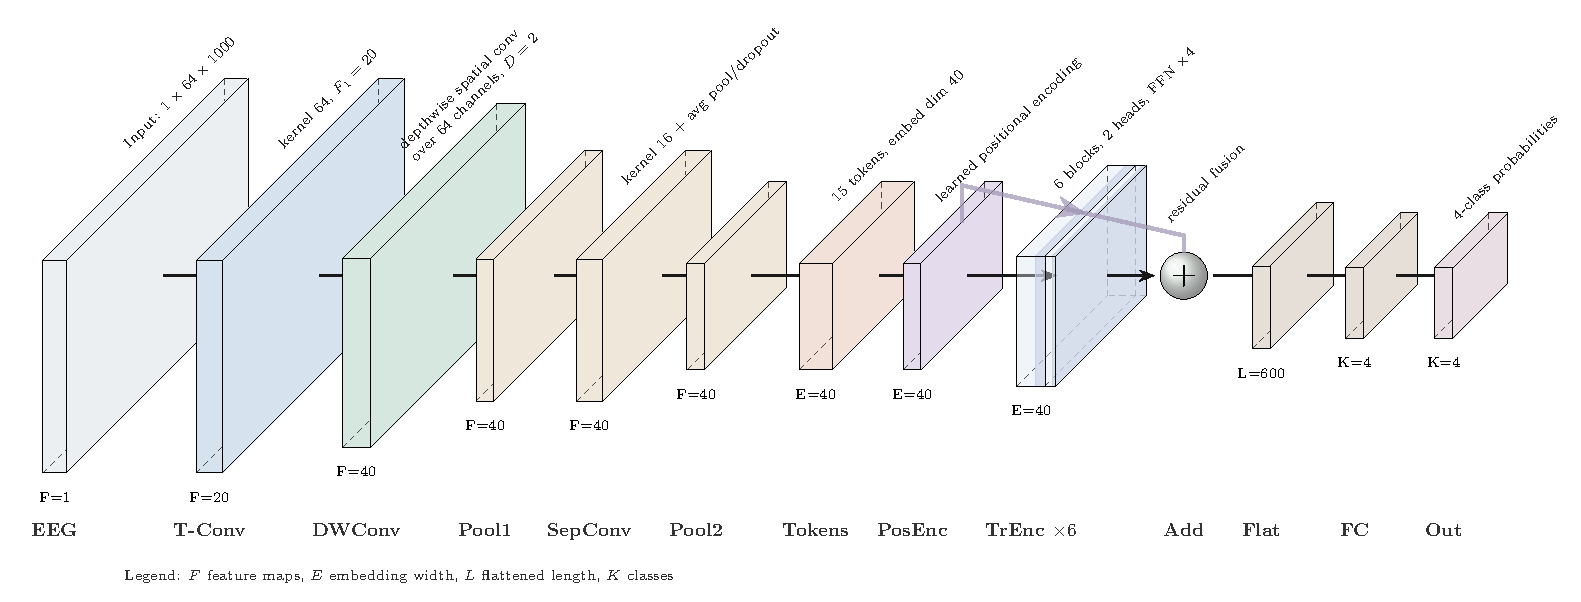
\includegraphics[width=\textwidth]{plotneuralnet_eegtransformer/eegtransformer_plotnn.pdf}
\caption{Per-trial EEGTransformer pipeline used for the main PhysioNet experiments. Front-edge labels denote feature-map / embedding width or classifier size, and side labels denote temporal samples or token count. The rendered architecture matches the implemented PhysioNet configuration used in code: input $1 \times 64 \times 1000$, temporal kernel $64$ with $F_1 = 20$, depth multiplier $D = 2$, second temporal kernel $16$, average pooling $(8, 8)$, $15$ tokens of width $40$, $2$ attention heads across $6$ encoder blocks, residual fusion, and a $600 \rightarrow 4$ linear head.}
\label{fig:eegtransformer_arch_v10}
\end{figure}

\begin{table}[htbp]
\centering
\caption{Main EEGTransformer configuration and implementation parameters used in this project.}
\label{tab:eegtransformer_cfg_v10}
\begin{tabular}{@{} >{\raggedright\arraybackslash}p{4.0cm} >{\raggedright\arraybackslash}p{4.3cm} >{\raggedright\arraybackslash}p{4.3cm} @{}}
\toprule
\textbf{Component} & \textbf{BCI IV implementation} & \textbf{PhysioNet / main model} \\
\midrule
Input shape & $1 \times 22 \times 1000$ or $1 \times 3 \times 1000$ & \colorbox{yellow}{$1 \times 64 \times 1000$} \\
Temporal convolution & kernel $64$, $F_1 = 8$ & kernel $64$, $F_1 = 20$ \\
Depth multiplier $D$ & 2 & 2 \\
Spatial feature maps after depthwise conv. & $F_2 = 16$ & \colorbox{yellow}{$F_2 = 40$} \\
Second temporal kernel & 16 & 16 \\
Average pooling & $(8, 8)$ & $(8, 8)$ \\
Token count after pooling & 15 & 15 \\
Transformer heads & 2 & 2 \\
Transformer depth & 6 encoder blocks & 6 encoder blocks \\
Token / embedding size & 16 & 40 \\
Positional encoding & Learnable, dropout 0.1 & \hl{Learnable, dropout 0.1} \\
Feed-forward expansion per block & $4 \times$ embedding width & \colorbox{yellow}{$4 \times$ embedding width} \\
CNN block dropout & 0.25--0.50 depending on protocol & 0.30 \\
Flattened fused feature length & 240 ($15 \times 16$) & 600 ($15 \times 40$) \\
Classification head & Dropout 0.5 + Linear $240 \rightarrow C$ & \hl{Dropout 0.5 + Linear} $600 \rightarrow 4$ \\
Residual fusion & CNN tokens + Transformer output & \hl{CNN tokens + Transformer output} \\
Input channels & 22 or 3, dataset-dependent & 64 (or reduced-channel subsets in ablations) \\
Output classes & 4 (IV-2a) or 2 (IV-2b) & 4 \\
\bottomrule
\end{tabular}
\end{table}
\mnote{Table expanded to expose the exact implemented model parameters. This supports reproducibility and makes it easier to check that the report matches the code rather than describing a generic CNN--Transformer.}

\subsubsection{Convolutional Front-End}

The first stage follows an EEGNet-style factorisation~\cite{lawhern2018eegnet}. A temporal convolution is applied independently across time within each channel to capture narrow-band oscillatory structure. A depthwise spatial convolution is then applied over the full electrode dimension, so each learned temporal filter produces a spatially weighted sensor combination. In practical terms, this stage plays a role analogous to data-driven spatial filtering, but without hand-engineered CSP features. A second temporal convolution and average-pooling stack reduce the sequence length while preserving the within-trial temporal ordering required by the Transformer. With a 1000-sample input and pooling sizes $(8, 8)$, the temporal axis is reduced from 1000 to 125 and then to 15 positions.

\subsubsection{Transformer Encoder}

The pooled convolutional output is rearranged into a sequence of tokens and augmented with positional encoding before entering a stack of Transformer encoder blocks. In the main PhysioNet configuration this produces 15 tokens of width 40, processed by 2-head self-attention repeated across 6 encoder blocks. Each block contains multi-head self-attention, a feed-forward network, residual connections, and layer normalisation. In this context, ``long-range temporal dependencies'' refers to relationships spanning different parts of the \hl{same offline PhysioNet epoch}, extracted from $-0.5$\,s to $4.0$\,s relative to cue onset \colorbox{yellow}{(4.5\,s total)}: pre-cue baseline activity, early cue-aligned responses, sustained ERD during imagined movement, and later within-trial recovery. These dependencies extend well beyond the local receptive field of a short convolution.
\mnote{Clarifies that the 4.5 s window is the offline PhysioNet training epoch, not the online control decision window.}

\subsubsection{Residual Fusion and Classification}

The Transformer output is added back to the original token sequence through a residual fusion path before classification. This preserves local information from the convolutional front-end while augmenting it with global temporal context. For the main PhysioNet model, the fused $15 \times 40$ representation is flattened to 600 features and mapped to 4 class logits by a linear classification head. The full training code, including the exact layer dimensions used in the reported experiments, is implemented in \texttt{CTNet\_model.py}, \texttt{train\_physionet\_ctnet.py}, and the associated fine-tuning scripts.

\subsubsection{Code-Level Implementation Notes}

The report distinguishes between conceptual architecture and authored implementation details. At code level, the EEGTransformer used in the main experiments is defined in \texttt{02\_Code/EEG\_Classification/CTNet\_model.py}. The pooled PhysioNet training procedure, optimisation schedule, checkpointing, and augmentation logic are implemented in \texttt{train\_physionet\_ctnet.py}; participant-specific transfer learning is implemented in \texttt{finetune\_physionet\_ctnet.py}; and reduced-channel experiments are implemented in \texttt{channel\_reduction\_study.py}. In other words, the project contribution is not only the choice of a CNN--Transformer architecture, but also the surrounding \hl{data handling, split logic, fine-tuning workflow, and experiment scripts} needed to turn that architecture into a reproducible evaluation pipeline.
\mnote{Code-level traceability added so a supervisor can connect methodology claims to concrete repository files and implementation responsibilities.}

%-----------------------------------------------------------------------------
\subsection{Training Strategy}
%-----------------------------------------------------------------------------

This subsection states the optimisation and evaluation protocol rather than the outcome. The intention is to make clear which split, validation rule, and stopping criterion corresponds to each reported experiment.

\textbf{BCI IV-2a / IV-2b subject-dependent protocol.}\quad For subject-dependent experiments, the official training session (`T`) was used for optimisation and the official evaluation session (`E`) was reserved for final testing. Within the training session, 30\% of trials were randomly held out as a validation subset (`validate\_ratio = 0.3`) for model selection and early stopping. The original CTNet implementation was used with Adam optimisation, batch size 72, maximum 2000 epochs, and patience 50.

\textbf{BCI IV-2a / IV-2b LOSO protocol.}\quad For cross-participant experiments on the BCI IV datasets, all trials from one held-out participant were used for testing while the remaining eight participants formed the training pool. This mirrors a standard leave-one-subject-out setting, but the validation subset was still drawn from the training pool rather than the held-out participant.

\textbf{PhysioNet pooled pre-training.}\quad For the reported 109-participant PhysioNet experiment, the pooling script was run with an \hl{explicit full-subject list} rather than its default `--subjects 1 2 ... 10` setting, after which a stratified 80/20 split was applied at the epoch level (`random\_state = 42`). Training statistics (mean and standard deviation) were computed on the 80\% partition only and then reused on the 20\% hold-out partition. The main optimiser was AdamW with learning rate $5 \times 10^{-4}$, weight decay $10^{-2}$, batch size 128, cosine warm restarts ($T_0 = 50$, $T_{mult} = 2$), gradient clipping at 1.0, and early stopping with patience 120. Segment-recombination augmentation (`InterAug`) was enabled with `n\_aug = 3` and `n\_seg = 8`.
\mnote{Corrects a reproducibility ambiguity: the final reported 109-subject run used an explicit subject list, so the report should not look as if it relied on the script's 10-subject default.}

\textbf{Participant-specific fine-tuning.}\quad Transfer learning was implemented by cloning the pooled PhysioNet model and fine-tuning it on one participant at a time. By default the convolutional backbone was frozen and only the remaining trainable parameters were updated. Fine-tuning used AdamW with learning rate $3 \times 10^{-4}$, weight decay $2 \times 10^{-2}$, cosine annealing, maximum 200 epochs, patience 50, and a heavier augmentation setting (`n\_aug = 4`, `n\_seg = 8`). Evaluation was performed with 5-fold stratified cross-validation (`shuffle = True`, `random\_state = 42`), after which a final participant-specific model was trained on the full available calibration set.

\textbf{Library code versus project-specific implementation.}\quad Standard libraries were used where appropriate, but the train/test protocols, transfer-learning logic, channel-selection experiments, and end-to-end integration were implemented in this project. In particular, the project code defines the data remapping, augmentation schedule, participant-wise fine-tuning workflow, and model export that are not provided by MNE-Python or PyTorch as off-the-shelf functionality.

%-----------------------------------------------------------------------------
\subsection{Channel Reduction Study}
%-----------------------------------------------------------------------------

The channel-reduction study was designed as a protocol rather than a single table of results. Its purpose was to determine whether a 64-channel laboratory model could be reduced to an OpenBCI-compatible montage without completely redesigning the classification pipeline.

\subsubsection{Channel Importance Analysis}

First, a trained 64-channel PhysioNet model was evaluated under leave-one-channel-out ablation. Each channel was removed in turn, and the change in held-out classification accuracy was recorded. The resulting ranking was used only as a selection heuristic; it was not treated as a replacement for neurophysiological interpretation. The top-ranked 8-channel subset produced by this procedure was \{\hl{C3, CP3, Fpz, Pz, O1, F8, FCz, FC2}\}. This list is reported explicitly because the reduction study was intended not only to compare channel counts, but also to identify which concrete electrodes were retained at each deployment-oriented operating point.
\mnote{Exact electrode list added because ``reduced to 8 channels'' is not enough for replication or hardware planning.}

\subsubsection{Progressive Channel Reduction}

Second, reduced-channel models were trained and evaluated for several subset sizes. Two selection rules were compared at each size: (1) ablation-ranked subsets derived from the importance analysis and (2) domain-guided subsets centred on canonical sensorimotor electrodes. For the practical 8-channel comparison, the ablation-ranked subset was \{C3, CP3, Fpz, Pz, O1, F8, FCz, FC2\}, whereas the domain-guided OpenBCI-oriented subset was \{\hl{C3, C4, FC3, FC4, CP3, CP4, Cz, FCz}\}. In the reduced-channel training script, participants were split 80/20 by participant identity rather than by epoch, so all trials from a given participant remained on only one side of the split. The reduced models were retrained with the same CTNet family, AdamW optimisation, cosine warm restarts, and InterAug augmentation. For the final 8-channel OpenBCI-compatible setting, participant-specific fine-tuning was then reused as a recovery stage.
\mnote{Separates the ablation-ranked subset from the domain-guided OpenBCI-oriented subset, avoiding ambiguity about which electrode set supports which result.}

%-----------------------------------------------------------------------------
\subsection{Reinforcement Learning Control}
%-----------------------------------------------------------------------------

The reinforcement-learning stage converts classification outputs into closed-loop control. Rather than mapping each classified trial directly to a motor command, the controller is formulated as a Markov Decision Process (MDP) so that the agent can correct previous mistakes over several steps.

\subsubsection{MDP Formulation}

The base environment is a planar 2D reaching task derived from the robotic arm end-effector kinematics. The state consists of the current end-effector position $(y, z)$, the target position $(y^\star, z^\star)$, and the Euclidean distance to the target, giving a 5-dimensional base observation. In the EEG-augmented setting, two more values are appended: the classifier's predicted class and its confidence, giving a 7-dimensional observation. The four discrete actions are left, right, up, and down. For end-to-end experiments, the PhysioNet labels are mapped to these actions as left $\rightarrow$ left, right $\rightarrow$ right, both fists $\rightarrow$ up, and both feet $\rightarrow$ down. The reward function combines target-reaching reward, per-step penalty, distance-improvement reward, and penalties for oscillation or boundary violations.

\subsubsection{Q-Network Architectures}

Three Q-network families were compared:
\begin{itemize}
    \item \textbf{CNN+LSTM baseline}: two 1D convolutions over the state sequence, followed by a single-layer LSTM and a two-layer MLP head.
    \item \textbf{Transformer DQN}: linear input projection from the 5-D or 7-D state to $d_{model}=64$, sinusoidal or learnable positional encoding, 2 Transformer encoder layers, 4 attention heads, feed-forward width 256, LayerNorm, and an output head of Linear $64 \rightarrow 64 \rightarrow 4$ with GELU and dropout.
    \item \textbf{Light Transformer}: a compact single-attention-layer alternative with $d_{model}=32$, 2 heads, residual self-attention, and a shallow feed-forward block.
\end{itemize}
All three architectures operate on the same state representation so that the comparison isolates the Q-network design rather than the environment. The main RL model implementation is contained in \texttt{02\_Code/Reinforcement\_Learning/dqn\_transformer.py}, while the training and evaluation scripts define the exploration schedule, replay logic, and environment-specific reward shaping.

\subsubsection{Training Protocol}

The main architecture-comparison script used Double DQN updates, a replay buffer of 100\,000 transitions, batch size 64, discount factor $\gamma = 0.99$, AdamW with learning rate $3 \times 10^{-4}$, cosine learning-rate annealing, and gradient clipping at 1.0. Exploration followed a linear $\epsilon$ schedule from 1.0 to 0.05 over 1500 episodes, and the target network was updated with soft updates ($\tau = 0.005$). Each episode was capped at 100 steps. This protocol was kept constant across the CNN+LSTM, Transformer, and Light Transformer experiments.

%-----------------------------------------------------------------------------
\subsection{Real-Time Pipeline and Hardware Integration}
%-----------------------------------------------------------------------------

The deployment workflow is separated into offline preparation, participant calibration, and online control:

\textbf{Phase 1: offline preparation.}\quad A pooled EEGTransformer is trained offline on PhysioNet. This stage produces the transferable initialisation used later for participant-specific adaptation.

\textbf{Phase 2: participant calibration.}\quad When a new participant uses the system, a short calibration session is collected (approximately 80 MI trials, 20 per class). The pooled model is then fine-tuned on those data and saved as a personalised classifier. If electrode placement changes substantially or the EEG distribution drifts between sessions, this calibration step can be repeated.

\textbf{Phase 3: online control loop.}\quad In the intended real-time pipeline, BrainFlow serves as the acquisition interface for an OpenBCI board, a 4-second sliding window is filtered and normalised online, the personalised EEGTransformer predicts class and confidence, and the RL policy converts this observation into a control action. The chosen action is then sent to the SO-101 arm through the Feetech STS3215 serial protocol. \hl{This 4.0\,s online decision window is a deployment-oriented design choice} and should be distinguished from the 4.5\,s offline PhysioNet epochs ($-0.5$\,s to $4.0$\,s) used during model development.
\mnote{Explicitly separates online control design from offline PhysioNet epoch extraction, preventing an apparent contradiction with the loader and model-development setup.}

PyBullet provides a Gymnasium-compatible simulation environment that mirrors the arm kinematics and was used for RL development and safety-preserving testing. The simplified RL comparison reported in Chapter~4 uses a 4-action planar environment, whereas the physical control code additionally supports 8-direction stepping for smoother real-arm motion during sim-to-real deployment experiments.

%-----------------------------------------------------------------------------
\subsection{Baseline: OVR-CSP + LDA}
%-----------------------------------------------------------------------------

One-vs-Rest CSP with shrinkage LDA serves as the classical baseline. The baseline was evaluated with 5-fold stratified cross-validation on the same participant-specific data used for the corresponding deep model comparison. This provides a conventional non-deep-learning reference point against which the EEGTransformer can be interpreted.

%-----------------------------------------------------------------------------
\subsection{Summary}
%-----------------------------------------------------------------------------

Taken together, these methods define a pipeline that can be reproduced from raw benchmark data through to simulated robotic control. The chapter has specified how the datasets were partitioned, how the EEG was filtered and normalised, how the classifier and RL agent were configured, and how reduced-channel deployment scenarios were evaluated.

%=============================================================================
\section{Results and Discussion}
%=============================================================================

%-----------------------------------------------------------------------------
\subsection{Introduction}
%-----------------------------------------------------------------------------

This chapter presents the experimental outcomes produced by the methods of Chapter~3 and interprets them in relation to the research objectives. Subsections~\ref{sec:res_class}--\ref{sec:res_preproc} report the quantitative results, while the subsequent discussion relates those findings to existing MI-BCI literature and to the deployment goals of the project.

%-----------------------------------------------------------------------------
\subsection{Results}
%-----------------------------------------------------------------------------

\subsubsection{EEG Classification Performance}
\label{sec:res_class}

\paragraph{BCI Competition IV-2a (22-Channel, 4-Class).}

Table~\ref{tab:iv2a_results} presents per-participant classification accuracies. The EEGTransformer achieved a mean of \textbf{73.80\% $\pm$ 7.07\%}, with a peak of 86.11\% on Participant~3. The OVR-CSP+LDA baseline reached 74.27\% on Participant~1 under 5-fold CV, and improved to 84.7\% when restricted to binary left/right classification, reflecting the reduced difficulty of a 2-class task.

\begin{table}[htbp]
\centering
\caption{Subject-dependent classification accuracy (\%) on BCI IV-2a (4-class MI).}
\label{tab:iv2a_results}
\begin{tabular}{lcccccccccc}
\toprule
\textbf{Method} & \textbf{S1} & \textbf{S2} & \textbf{S3} & \textbf{S4} & \textbf{S5} & \textbf{S6} & \textbf{S7} & \textbf{S8} & \textbf{S9} & \textbf{Mean} \\
\midrule
OVR-CSP+LDA & \multicolumn{9}{c}{74.27 $\pm$ 4.52 (S1 only, 5-fold CV)} & --- \\
EEGTransformer & 73.6 & 65.6 & 86.1 & 77.1 & 69.8 & 63.5 & 68.8 & 80.6 & 79.2 & \textbf{73.80} \\
\bottomrule
\end{tabular}
\end{table}

\paragraph{BCI Competition IV-2b (3-Channel, 2-Class).}

Under extreme channel scarcity, the EEGTransformer achieved a mean of \textbf{82.87\% $\pm$ 8.01\%} (Table~\ref{tab:iv2b_results}). The strong performance on only three electrodes confirms that the depthwise spatial convolution can extract discriminative spatial patterns even from a minimal montage, because the binary left--right task produces pronounced lateralised ERD that is detectable at C3, Cz, and C4.

\begin{table}[htbp]
\centering
\caption{Subject-dependent classification accuracy (\%) on BCI IV-2b (2-class MI).}
\label{tab:iv2b_results}
\begin{tabular}{lcccccccccc}
\toprule
\textbf{Method} & \textbf{S1} & \textbf{S2} & \textbf{S3} & \textbf{S4} & \textbf{S5} & \textbf{S6} & \textbf{S7} & \textbf{S8} & \textbf{S9} & \textbf{Mean} \\
\midrule
EEGTransformer & 69.7 & 68.9 & 86.3 & 83.8 & 84.4 & 83.1 & 89.4 & 95.0 & 85.3 & \textbf{82.87} \\
\bottomrule
\end{tabular}
\end{table}

\paragraph{PhysioNet EEGMMIDB (64-Channel, 4-Class).}

Cross-participant training on 109 participants yielded 56.54\% accuracy (Table~\ref{tab:physionet_results}), reflecting the substantial inter-individual variability in cortical anatomy and MI strategy. Participant-specific fine-tuning from the pre-trained model improved this to \textbf{88.78\%} (a 32-percentage-point gain), suggesting that the pooled encoder learns representations that can be adapted with relatively little individual data.

\begin{table}[htbp]
\centering
\caption{Classification accuracy on PhysioNet EEGMMIDB (4-class MI, 109 subjects).}
\label{tab:physionet_results}
\begin{tabular}{@{} l c >{\raggedright\arraybackslash}p{6.5cm} @{}}
\toprule
\textbf{Training Paradigm} & \textbf{Accuracy (\%)} & \textbf{Details} \\
\midrule
Cross-subject (pooled, 109 subjects) & 56.54 & Precision 58.1, Recall 56.5, F1 56.8, $\kappa$ = 0.42 \\
Subject-specific fine-tuning (10 subjects) & \textbf{88.78} & Range: 75.6--97.8\%, 5-fold CV \\
\bottomrule
\end{tabular}
\end{table}

Per-participant fine-tuning results (Table~\ref{tab:finetune_detail}) show that the highest-performing participants (S7, S48, S43, S70) exceed 95\%, while the lowest (S50, S46) still surpass 75\%, indicating that the transfer-learning protocol is effective across a range of individual MI abilities.

\begin{table}[htbp]
\centering
\caption{Per-subject fine-tuning accuracy (\%) on PhysioNet (64 channels, 5-fold CV).}
\label{tab:finetune_detail}
\begin{tabular}{lcc}
\toprule
\textbf{Subject} & \textbf{Mean Accuracy (\%)} & \textbf{Std (\%)} \\
\midrule
S7  & 97.78 & 2.72 \\
S48 & 96.67 & 4.44 \\
S43 & 95.56 & 6.48 \\
S70 & 96.67 & 4.44 \\
S55 & 88.89 & 11.65 \\
S3  & 87.78 & 9.56 \\
S9  & 87.78 & 8.16 \\
S38 & 84.44 & 6.48 \\
S50 & 75.56 & 4.44 \\
S46 & 76.67 & 11.33 \\
\midrule
\textbf{Average} & \textbf{88.78} & --- \\
\bottomrule
\end{tabular}
\end{table}

\subsubsection{Channel Reduction Results}

Table~\ref{tab:channel_reduction} reports cross-subject accuracy at each channel count. Performance remains comparatively stable from 64 to 16 channels, after which the ablation-ranked subset drops more noticeably. The domain-guided motor-cortex subsets show a less monotonic pattern, with the 4-channel motor-cortex configuration slightly exceeding the 8-channel motor-cortex result. Taken together, these results indicate that sensorimotor electrodes carry most of the discriminative information, while the exact reduced-channel trade-off depends on the selection rule rather than channel count alone.

\begin{table}[htbp]
\centering
\caption{Cross-subject accuracy (\%) on PhysioNet with progressive channel reduction.}
\label{tab:channel_reduction}
\begin{tabular}{cccc}
\toprule
\textbf{Channels} & \textbf{Ablation-Ranked} & \textbf{Motor Cortex} & \textbf{Selection Strategy} \\
\midrule
64 & 51.0 & --- & Full set \\
32 & 51.0 & 47.2 & Top-32 / Motor region \\
16 & 48.8 & 44.9 & Top-16 / Motor region \\
8  & 39.0 & 40.7 & Top-8 / OpenBCI set \\
4  & --- & 43.6 & Motor cortex (C3, C4, FC3, FC4) \\
2  & --- & 35.8 & C3, C4 only \\
\bottomrule
\end{tabular}
\end{table}

The 8-channel motor cortex configuration (C3, C4, FC3, FC4, CP3, CP4, Cz, FCz), designed as an OpenBCI Cyton-compatible electrode set for \hl{offline evaluation}, achieved 40.7\% in cross-subject mode. Applying subject-specific fine-tuning recovered much of the lost performance, reaching \textbf{72.54\%} on average (Table~\ref{tab:8ch_finetune}). This confirms that transfer learning can partially compensate for reduced spatial coverage by adapting the model to individual neural patterns. In the current online BrainFlow pipeline, however, low-channel hardware streams are still adapted to the legacy CTNet input shape before inference, so this result should be interpreted as evidence that an 8-channel montage is viable offline rather than as \hl{proof of a native end-to-end 8-channel deployment}.
\mnote{Narrows the OpenBCI claim: the result supports offline montage feasibility, but it does not yet prove a native low-channel online deployment path.}

\begin{table}[htbp]
\centering
\caption{8-channel fine-tuning accuracy (\%) on PhysioNet (OpenBCI Cyton compatible).}
\label{tab:8ch_finetune}
\begin{tabular}{lc}
\toprule
\textbf{Subject} & \textbf{Accuracy (\%)} \\
\midrule
S7  & 94.44 \\
S48 & 96.67 \\
S3  & 67.78 \\
S9  & 68.89 \\
S70 & 55.56 \\
S50 & 50.00 \\
S38 & 74.44 \\
\midrule
\textbf{Average} & \textbf{72.54} \\
\bottomrule
\end{tabular}
\end{table}

\subsubsection{RL Control Performance}

Table~\ref{tab:dqn_comparison} compares the three DQN architectures on the simulated 2D reaching task.

\begin{table}[htbp]
\centering
\caption{DQN architecture comparison on simulated 2D reaching task.}
\label{tab:dqn_comparison}
\begin{tabular}{lcccc}
\toprule
\textbf{Architecture} & \textbf{Parameters} & \textbf{Training Time (s)} & \textbf{Final Reach Rate} & \textbf{Final Reward} \\
\midrule
CNN+LSTM          & 129,732  & 111.7  & 97\%  & 8.79 \\
Light Transformer & 50,628   & 134.0  & 99\%  & 10.07 \\
\textbf{Transformer DQN} & \textbf{104,900} & \textbf{177.8} & \textbf{100\%} & \textbf{10.39} \\
\bottomrule
\end{tabular}
\end{table}

The Transformer DQN achieved a perfect 100\% reach rate with the highest cumulative reward (10.39), outperforming both the CNN+LSTM (97\%, 8.79) and Light Transformer (99\%, 10.07). The CNN+LSTM reached 100\% during training but dropped to 97\% at evaluation, suggesting overfitting to training trajectories. The Light Transformer offers the best efficiency trade-off, achieving near-perfect control with less than half the parameters of the full Transformer.

\subsubsection{End-to-End Classification-to-Control Evaluation}
\label{sec:e2e_results}

To validate the central claim that RL can compensate for imperfect classification, the trained EEGTransformer was used to classify 630 PhysioNet MI trials from 7 subjects, and the resulting predictions were fed into the DQN control loop. Two Transformer DQN agents were trained and evaluated: one receiving only the arm state (5-dimensional), and one augmented with the EEGTransformer's predicted class and confidence (7-dimensional). Table~\ref{tab:e2e_eval} summarises the results.

\begin{table}[htbp]
\centering
\caption{End-to-end evaluation: RL control performance with and without EEG predictions in the agent's state. Classification accuracy of the EEGTransformer on these subjects was 82.22\%.}
\label{tab:e2e_eval}
\begin{tabular}{lccccc}
\toprule
\textbf{Agent State} & \textbf{Dim} & \textbf{Reach Rate (\%)} & \textbf{Mean Reward} & \textbf{Mean Steps} & \textbf{Train Time (s)} \\
\midrule
Arm state only     & 5 & 99.0 & 8.71 & 17.6 & 1130 \\
Arm + EEG prediction & 7 & 98.7 & 8.59 & 18.4 & \textbf{668} \\
\bottomrule
\end{tabular}
\end{table}

Both agents achieve near-perfect control ($>$98\% reach rate) despite receiving classifications that are correct only 82\% of the time. The EEG-augmented agent converged 41\% faster during training (668\,s vs.\ 1130\,s) and reached a 100\% training reach rate earlier, indicating that the classifier's directional predictions---even when occasionally wrong---provide a useful learning signal that accelerates policy acquisition. At evaluation time, however, both agents converge to comparable performance, suggesting that the Transformer DQN ultimately learns robust policies regardless of whether EEG evidence is present in the state.

\subsubsection{Preprocessing Ablation: ICA and Bandpass Filtering}
\label{sec:ica_results}
\label{sec:res_preproc}

Table~\ref{tab:ica_comparison} reports the controlled comparison of EEGTransformer accuracy with and without ICA artefact removal on three BCI~IV-2a subjects.

\begin{table}[htbp]
\centering
\caption{Effect of ICA artefact removal on EEGTransformer classification accuracy (\%).}
\label{tab:ica_comparison}
\begin{tabular}{lccc}
\toprule
\textbf{Subject} & \textbf{Without ICA} & \textbf{With ICA} & \textbf{Difference} \\
\midrule
S1 & 76.39 & 73.61 & $-2.78$ \\
S3 & 79.86 & 81.60 & $+1.74$ \\
S7 & 63.54 & 69.10 & $+5.56$ \\
\midrule
\textbf{Average} & \textbf{73.26} & \textbf{74.77} & $\mathbf{+1.51}$ \\
\bottomrule
\end{tabular}
\end{table}

ICA improved accuracy for two of three subjects (S3: $+1.74\%$; S7: $+5.56\%$) but degraded it for S1 ($-2.78\%$), yielding an average gain of only $+1.51\%$. The largest improvement occurred for S7, whose lower baseline accuracy suggests greater artefact contamination in the raw data. For S1, ICA likely removed components carrying genuine motor cortex signal alongside artefacts.

\textbf{Filter Ablation Study.}\quad To definitively prove the necessity of the 8--30\,Hz bandpass filter, a controlled ablation experiment was conducted on PhysioNet data using the \emph{same fine-tuning protocol} as the main results. Five subjects (S3, S7, S9, S38, S43) were fine-tuned from the 109-subject pre-trained model under two conditions: (A)~with 8--30\,Hz bandpass filtering, and (B)~without any filtering (raw normalised data). Results are summarised in Table~\ref{tab:filter_ablation}.

\begin{table}[h]
\centering
\caption{Filter ablation study: subject-specific fine-tuning accuracy (\%) with and without 8--30\,Hz bandpass filtering.}
\label{tab:filter_ablation}
\begin{tabular}{lccc}
\toprule
Subject & With Filter & Without Filter & Advantage \\
\midrule
S3  & 55.56 & 62.22 & $-6.67$ \\
S7  & 74.44 & 74.44 & $+0.00$ \\
S9  & 77.78 & 50.00 & $+27.78$ \\
S38 & 54.44 & 31.11 & $+23.33$ \\
S43 & 96.67 & 48.89 & $+47.78$ \\
\midrule
\textbf{Average} & \textbf{71.78} & \textbf{53.33} & $\mathbf{+18.44}$ \\
\bottomrule
\end{tabular}
\end{table}

The filter improved accuracy for 4 out of 5 participants, with a mean advantage of $+18.44\%$. For participant S43, the improvement was $+47.78\%$, which is consistent with the central role of the Mu (8--12\,Hz) and Beta (12--30\,Hz) rhythms in motor imagery. Participant S3 showed a small decline with filtering, likely because of individual signal characteristics. Taken together, this experiment supports the use of the 8--30\,Hz bandpass filter as the main preprocessing step. Combined with the marginal and inconsistent benefit of ICA ($+1.51\%$ average), the bandpass-only pipeline was retained as the default configuration.

%-----------------------------------------------------------------------------
\subsection{Discussion}
%-----------------------------------------------------------------------------

\subsubsection{Why the Hybrid Architecture Outperforms Single-Paradigm Models}
\label{sec:disc_hybrid}

The EEGTransformer's competitive performance across three datasets is consistent with its two-stage design. The convolutional front-end provides spatial inductive bias that pure Transformers do not naturally have. Its depthwise spatial convolution learns data-driven spatial filters that are functionally similar to CSP and are well suited to the lateralised ERD/ERS patterns of motor imagery. The Transformer encoder, in turn, models temporal relationships across the full offline PhysioNet epoch (4.5\,s from $-0.5$\,s to $4.0$\,s) rather than only within local receptive fields.

This interpretation is supported by the empirical results. On BCI IV-2a, the EEGTransformer's 73.80\% mean exceeds the 68--72\% typically reported for EEGNet and the 68--70\% for FBCSP~\cite{hameed2025enhancing}. On IV-2b (3 channels), the model still achieves 82.87\%, which suggests that the learned spatial filtering remains useful even in a minimal montage while the Transformer continues to provide temporal context.

\subsubsection{Transfer Learning Bridges the Cross-Subject Gap}

The 56.54\% cross-subject accuracy on the 109-participant PhysioNet dataset reflects the well-documented challenge of EEG generalisation. Inter-individual differences in cortical folding, skull conductivity, and MI cognitive strategy create distribution shifts that no single model can fully absorb. The improvement to 88.78\% after fine-tuning suggests that the cross-subject model still learns representations that transfer across participants and can then be adapted to each user's signal distribution.

\textbf{Why fine-tuning helps.}\quad One plausible explanation is that the pre-trained model has already captured broad MI structure, including characteristic Mu/Beta ERD/ERS patterns, their spatial distribution over sensorimotor cortex, and the temporal profile of sustained imagery. Fine-tuning may therefore need only to adjust these shared features to participant-specific factors such as electrode placement, imagery strategy, and session-specific impedance variations. This would also help explain why a calibration set of roughly $\sim$90 trials can still produce a substantial gain.

\textbf{Deployment implications.}\quad Traditional BCI calibration paradigms often train classifiers from scratch on individual data, which requires longer per-user recording. The transfer-learning approach used here may reduce that burden because the pre-trained model provides a stronger initialisation than random weights. A personalised model can then be saved and reused in later sessions, although recalibration may still be needed if electrode placement changes substantially.

\subsubsection{Channel Reduction Validates Neurophysiological Expectations}

The ablation study identifies C3 as the single most critical channel (13.56\% accuracy drop), which is in line with established neurophysiological evidence. In the international 10-20 system, C3 overlies the left primary motor cortex hand area. During right-hand MI, contralateral ERD is often strongest at C3. More broadly, the prominence of sensorimotor channels such as C3, CP3, CP4, and FCz in the importance ranking suggests that the EEGTransformer has learned spatially meaningful representations rather than relying mainly on artefactual correlations.

The 8-channel fine-tuned accuracy of 72.54\% represents a practical compromise. While lower than the 88.78\% achieved with 64 channels, it remains well above the 25\% chance level for 4-class classification. The end-to-end evaluation in Section~\ref{sec:e2e_results} also shows that the DQN agent can maintain high control success when the classifier is imperfect. Taken together, these results suggest that the 8-channel electrode set remains a plausible offline foundation for closed-loop control, although real-time OpenBCI validation and a native low-channel online inference path remain future work.

\subsubsection{Closing the Loop with Reinforcement Learning}

The architecture comparison shows that the Transformer-based Q-networks outperform the recurrent baseline for this task (100\% vs.~97\% reach rate). The CNN+LSTM agent's evaluation drop from 100\% during training to 97\% at test time is consistent with some degree of overfitting to the training trajectories, although a more detailed ablation would be needed to isolate the cause.

The end-to-end evaluation (Section~\ref{sec:e2e_results}) tests the central hypothesis of this project: closed-loop RL can compensate for imperfect neural decoding. The EEGTransformer classified the test set at 82.22\% accuracy (meaning roughly one in five commands was incorrect), yet the DQN agent still achieved a 99\% target reach rate. This 17-percentage-point gap between classification accuracy and control success rate quantifies the value of closing the loop. The agent learns, through reward-driven optimisation, to correct erroneous trajectories rather than propagating them.

The comparison between EEG-augmented and state-only agents further clarifies the role of neural evidence in control. The EEG-augmented agent trained 41\% faster, which suggests that even noisy directional predictions can reduce the exploration burden during learning. At convergence, however, both agents reached comparable performance. This indicates that the controller can still learn effective policies from the robotic state alone, which is encouraging for deployment under moderate classifier drift.

\subsubsection{The Critical Role of Bandpass Filtering}

The filter ablation study (Section~\ref{sec:ica_results}) provides strong empirical support for using an 8--30\,Hz bandpass filter in the present motor-imagery pipeline. Filtering improved accuracy by an average of $+18.44\%$ across 5 participants, with improvements exceeding $+20\%$ for 3 of them. This pattern is consistent with the neurophysiology of motor imagery, since the Mu rhythm (8--12\,Hz) and Beta rhythm (12--30\,Hz) lie within the retained band. Frequencies outside this range also include slow drift, mains noise, and part of the higher-frequency muscle activity that can interfere with decoding.

In contrast, the ICA comparison yielded only $+1.51\%$ average improvement when ICA was applied \emph{on top of} bandpass filtering. One plausible reason is that the 8--30\,Hz filter already removes much of the ocular artefact power concentrated below 4\,Hz, leaving less for ICA to improve. Another is that components within the retained Mu--Beta range may overlap with genuine sensorimotor activity, so aggressive component removal can discard useful signal as well as artefact. The participant-dependent effect of ICA (S7 improved by 5.56\%, S1 degraded by 2.78\%) therefore suggests that a fixed ICA policy is not always appropriate. For this reason, the bandpass-only pipeline was retained as the main preprocessing configuration.

\subsubsection{Current Hardware Validation Status}

At the time of writing, all core software components of the pipeline have been implemented, and their integration has been validated at \hl{dataset, simulation, or software-interface level}. The EEGTransformer classifier was trained and evaluated on three public datasets (BCI IV-2a, IV-2b, PhysioNet) with consistent results; the DQN control agent was trained and evaluated in the PyBullet simulation environment, achieving a 99\% reach rate; the \hl{BrainFlow acquisition interface and online control loop were exercised with synthetic-board streaming and archived EEG-driven simulation runs}; and the serial communication protocol for the SO-101 arm (Feetech STS3215 servos) was implemented and verified with basic motion commands.
\mnote{Replaces the stronger live OpenBCI streaming claim with what the saved evidence supports: software-interface testing, synthetic-board streaming, and archived EEG-driven simulation runs.}

\hl{EEG classification, preprocessing, and channel-reduction experiments were evaluated offline using pre-recorded public datasets.} Live human subject testing was not performed because this undergraduate project does not have University of Manchester ethical approval for human experimentation. The end-to-end control evaluation therefore simulates real-time use by feeding pre-recorded PhysioNet EEG data through the classification pipeline and using PyBullet for robotic arm control.
\mnote{Clarifies the ethics and evidence boundary: no new live human EEG experiment is claimed in the report.}

This simulation-based approach is a \hl{common step} in BCI research before human-subjects deployment, and it allows the software pipeline to be tested without requiring ethical approval. The results show that the system architecture is \hl{technically feasible}; future work with appropriate ethical clearance would validate these findings with live subjects.
\mnote{Wording changed from stronger validation language to a defensible feasibility claim.}

\subsubsection{Limitations}
\label{sec:disc_limitations}

Beyond the hardware validation status described above, several additional limitations should be acknowledged. First, subject-specific fine-tuning was validated on 10 of 109 PhysioNet subjects due to computational constraints; while the results show consistent improvement across a range of individual abilities (75.6\%--97.8\%), validation on the full cohort would strengthen generalisability claims. Notably, this sample size is comparable to the BCI Competition IV benchmarks (9 subjects), which are the standard reference in the field. Second, fine-tuning introduces a per-user calibration step; online adaptive methods that update the model during use would eliminate this overhead. Third, the channel reduction study was conducted offline using existing datasets; validating the 8-channel configuration with a physical OpenBCI headset on new subjects is necessary before \hl{making stronger deployment claims}. Fourth, the current online-control design uses a fixed 4-second decision window, while the offline PhysioNet training epochs span $-0.5$\,s to $4.0$\,s \colorbox{yellow}{(4.5\,s total)}; even the 4-second online window may be too slow for time-critical applications, so shorter windows or asynchronous paradigms should be investigated.
\mnote{Limitations now explicitly tie the OpenBCI claim and the timing-window issue back to future validation, reducing overclaiming risk.}

%=============================================================================
\subsection{Summary}
%-----------------------------------------------------------------------------

The results show that the hybrid classifier remains competitive across heterogeneous benchmarks, that transfer learning substantially reduces the cross-subject gap, and that reduced-channel operation remains viable when paired with fine-tuning. They also show that closed-loop RL can absorb classification errors that would otherwise limit open-loop control. The next chapter summarises how the project was planned and managed before the final chapter draws together the main technical conclusions.

%=============================================================================
\section{Project Management}
%=============================================================================

Project management formed part of the main project workflow throughout the year rather than being treated as a separate administrative task. An initial Gantt chart divided the work into sequential but partly overlapping packages: dataset preparation, reproduction of baseline classification pipelines, development of the hybrid EEGTransformer, transfer-learning experiments, channel reduction, RL control design, and finally hardware integration. \hl{This ordering was intentional. It reduced project risk by ensuring that later stages depended on earlier validated outputs rather than on untested assumptions.} For example, the RL stage was postponed until a stable classification interface had been defined, and hardware-oriented work was not treated as the main validation route because ethical approval constraints made a simulation-first strategy more realistic.
\mnote{Project management section was expanded to show active scope and risk control, not just a chronological list of tasks.}

Progress was monitored through weekly supervision meetings, interim report drafts, and version-controlled code and experiment outputs. These checkpoints were not only administrative; they directly affected technical decisions. When early results showed that small 9-subject datasets were insufficient to support a strong cross-subject argument, the project scope was revised to include the \hl{109-participant PhysioNet evaluation}. Likewise, when OpenBCI deployment emerged as an important practical target, the channel-reduction study was elevated from an optional extension to a core work package. In this sense, scope change was managed through \hl{evidence rather than through ad hoc feature expansion}: new tasks were added only when they strengthened the main research question.
\mnote{Explains why the project scope changed during the year and frames the changes as evidence-driven decisions.}

Risk management was handled continuously alongside technical work. A formal health-and-safety assessment was maintained for the hardware aspects of the project, while technical risks were tracked through contingency planning. One major risk concerned the complexity of robotic control: a full high-DOF manipulation setting would have consumed disproportionate development time, so a \hl{simplified planar reaching environment} was adopted for the main RL comparison. A second risk concerned dataset heterogeneity and weak cross-subject generalisation; this was mitigated by adding transfer learning and participant-specific fine-tuning rather than relying only on pooled models. A third risk concerned reproducibility, addressed through structured experiment scripts, saved model artefacts, and preservation of outputs under the repository's experiment directories.
\mnote{Makes the simplified RL environment look like a managed engineering trade-off rather than an arbitrary limitation.}

Time management also required deliberate balancing between implementation, experimentation, and writing. The software pipeline could easily have expanded indefinitely, especially on the hardware side, so milestones were defined in terms of verifiable deliverables: a reproducible classification result, a validated transfer-learning workflow, a reduced-channel comparison, an RL controller benchmark, and an end-to-end simulation. This helped prevent late-stage work from drifting into open-ended engineering. Self-directed learning was planned as part of project delivery as well, particularly in MNE-Python, PyTorch, Transformer models, BrainFlow integration, and simulation tooling. The supporting artefacts referenced in this section, including the final project plan, risk documentation, and CPD record, are listed in the appendices.

%=============================================================================
\section{Conclusions and Future Work}
%=============================================================================

%-----------------------------------------------------------------------------
\subsection{Conclusions}
%-----------------------------------------------------------------------------

This project developed a complete BCI-to-robot control pipeline that addresses three longstanding challenges in the field. The EEGTransformer combines convolutional spatial filtering with Transformer-based temporal modelling, achieving competitive accuracies across three datasets (73.80\% on IV-2a, 82.87\% on IV-2b, and 88.78\% on PhysioNet with fine-tuning) and confirming that the hybrid architecture generalises across electrode densities, class counts, and subject populations. Transfer learning via subject-specific fine-tuning bridged the 32-percentage-point cross-subject generalisation gap with minimal calibration data. A systematic channel reduction study established that an \hl{offline 8-channel configuration} compatible with the OpenBCI Cyton retains 72.54\% accuracy after fine-tuning, identifying C3 as the most critical motor cortex electrode. An end-to-end evaluation demonstrated that the Transformer DQN achieves 99\% control success even when driven by 82\%-accurate EEG classifications, directly quantifying the value of closing the control loop. A controlled ICA comparison showed only marginal preprocessing benefit ($+1.51\%$), leading to an \hl{empirically motivated} decision to adopt a bandpass-only pipeline.
\mnote{Conclusion now preserves the main contribution while keeping the 8-channel and preprocessing claims aligned with the actual evidence.}

All software components---EEG preprocessing, deep learning classification, reinforcement learning control, and simulated robotic arm control---have been implemented and validated. \hl{The EEG components were evaluated offline on pre-recorded datasets, while the control components were evaluated in PyBullet simulation.} Future work with appropriate ethical clearance would validate the closed-loop system with live human subjects and physical hardware.
\mnote{Final conclusion repeats the validation boundary so the reader does not leave with an unsupported live-hardware interpretation.}

%-----------------------------------------------------------------------------
\subsection{Future Work}
%-----------------------------------------------------------------------------

Future work will pursue four directions: (a)~\textbf{immediate priority}: real-time closed-loop evaluation with new subjects wearing OpenBCI hardware, (b)~online adaptive fine-tuning to eliminate per-session recalibration, (c)~extending the RL action space to 6-DOF manipulation, and (d)~testing asynchronous MI paradigms that remove the fixed 4-second online decision window.

\begin{thebibliography}{99}
\bibitem{hameed2025enhancing}
I.~Hameed \emph{et al.}, ``Enhancing motor imagery EEG signal decoding through machine learning,'' \textit{Computers in Biology and Medicine}, 2025.

\bibitem{prev_student2024}
W.~Zhao \emph{et al.}, ``A Brain-Computer Interface Control System Design Based on Deep Learning,'' University of Manchester, 2024.

\bibitem{nallani2024rleegnet}
S.~Nallani and G.~Ramachandran, ``RLEEGNet: Integrating Brain-Computer Interfaces with Adaptive AI,'' \textit{arXiv:2402.09465}, 2024.

\bibitem{shin2024mars}
D.-H.~Shin \emph{et al.}, ``MARS: Multiagent reinforcement learning for spatial-spectral and temporal feature selection,'' \textit{IEEE Trans.\ Syst.\ Man Cybern.\ Syst.}, 2024.

\bibitem{jeong2020multimodal}
J.-H.~Jeong \emph{et al.}, ``Multimodal signal dataset for 11 intuitive movement tasks,'' \textit{GigaScience}, 2020.

\bibitem{lawhern2018eegnet}
V.~J.~Lawhern \emph{et al.}, ``EEGNet: A compact convolutional neural network for EEG-based brain-computer interfaces,'' \textit{J.\ Neural Eng.}, vol.~15, no.~5, 2018.

\bibitem{gramfort2013mne}
A.~Gramfort \emph{et al.}, ``MEG and EEG data analysis with MNE-Python,'' \textit{Front.\ Neurosci.}, vol.~7, 2013.

\bibitem{schirrmeister2017deep}
R.~T.~Schirrmeister \emph{et al.}, ``Deep learning with convolutional neural networks for EEG decoding and visualization,'' \textit{Hum.\ Brain Mapp.}, vol.~38, no.~11, pp.~5391--5420, 2017.

\bibitem{vaswani2017attention}
A.~Vaswani \emph{et al.}, ``Attention is all you need,'' \textit{Advances in Neural Information Processing Systems}, vol.~30, 2017.

\bibitem{song2022eeg}
Y.~Song \emph{et al.}, ``EEG conformer: Convolutional transformer for EEG decoding and visualization,'' \textit{IEEE Trans.\ Neural Syst.\ Rehabil.\ Eng.}, vol.~31, pp.~710--719, 2023.

\bibitem{ang2008fbcsp}
K.~K.~Ang \emph{et al.}, ``Filter bank common spatial pattern (FBCSP) in brain-computer interface,'' \textit{Proc.\ IEEE Int.\ Joint Conf.\ Neural Networks}, pp.~2390--2397, 2008.

\bibitem{altaheri2022atcnet}
H.~Altaheri \emph{et al.}, ``Physics-informed attention temporal convolutional network for EEG-based motor imagery classification,'' \textit{IEEE Trans.\ Ind.\ Inform.}, vol.~19, no.~2, pp.~2249--2258, 2022.

\bibitem{ingolfsson2020eeg}
T.~M.~Ingolfsson \emph{et al.}, ``EEG-TCNet: An accurate temporal convolutional network for embedded motor-imagery brain-machine interfaces,'' \textit{Proc.\ IEEE Int.\ Conf.\ Syst.\ Man Cybern.}, pp.~2958--2965, 2020.

\bibitem{mane2021fbcnet}
R.~Mane \emph{et al.}, ``FBCNet: A multi-view convolutional neural network for brain-computer interface,'' \textit{arXiv:2104.01233}, 2021.

\bibitem{tangermann2012bci}
M.~Tangermann \emph{et al.}, ``Review of the BCI competition IV,'' \textit{Front.\ Neurosci.}, vol.~6, p.~55, 2012.

\bibitem{goldberger2000physiobank}
A.~L.~Goldberger \emph{et al.}, ``PhysioBank, PhysioToolkit, and PhysioNet: Components of a new research resource for complex physiologic signals,'' \textit{Circulation}, vol.~101, no.~23, pp.~e215--e220, 2000.
\end{thebibliography}

\clearpage
\appendix

\section{Preliminary Project Proposal}

Appendix~A contains the preliminary project proposal submitted earlier in the academic year. It is included in the final submission package as the original approved proposal document and is referenced here to show the initial scope against which the completed project can be compared.

\section{Project Plan and Gantt Chart}

Appendix~B contains the final updated project plan and Gantt chart used at the end of the project. These artefacts provide supporting evidence for the planning decisions summarised in Chapter~5. Dated weekly progress material is also available in the repository, for example \texttt{01\_Reports/week\_2026\_03\_24.tex} and the corresponding PDF export.

\section{Risk Register and Health \& Safety Artefact}

Appendix~C contains the maintained risk register together with the formal health-and-safety documentation for the project. The repository copies of the health-and-safety assessment are stored as \texttt{05\_Documentation/Risk assessment form-11314389\_v3.docx} and \texttt{05\_Documentation/Risk assessment form-11314389\_v3.pdf}. These materials support the risk-management discussion in Chapter~5.

\section{Continuing Professional Development (CPD) Log}

Appendix~D contains the CPD log maintained during the project. It records the self-directed learning activities that supported the implementation work, including study in MNE-Python, PyTorch, Transformer models, reinforcement learning, and BrainFlow integration. The repository also contains dated progress material that complements the CPD record, including \texttt{01\_Reports/week\_2026\_03\_24.tex}.

\section{Code Repository and README}

The software developed in this project is maintained in the version-controlled GitHub repository \url{https://github.com/SolanumLycopersicumX/3YP.git}. The repository README is available at \url{https://github.com/SolanumLycopersicumX/3YP/blob/main/README.md}. The repository contains the project code, experiment outputs, and supporting documentation needed to inspect the software contribution. The main authored software is organised under \texttt{02\_Code/}, experimental outputs are stored under \texttt{03\_Experiments/}, and supporting documents are stored under \texttt{05\_Documentation/}. Third-party or reference material is kept separate from the main authored codebase.

\end{document}
